\section{Results}

\begin{figure}
  \begin{centering}
  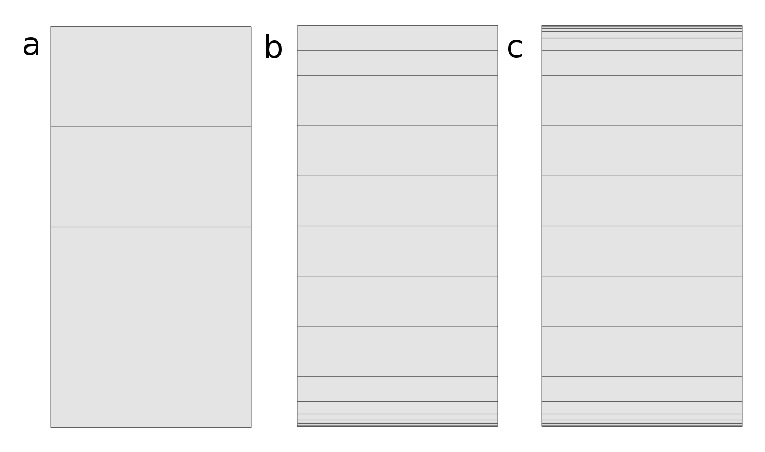
\includegraphics[width=.8\columnwidth]{mesh}
  \caption{\label{fig:mesh} Initial coarse mesh (a),
  	half refined mesh (b) and refined mesh (c). The coarse mesh
	and refined mesh were used in the initial calcualtions, the latter one
	in case of \emph{p}-adaptivity (including HP\_ANISO\_P). The half-refined mesh was
	used later to optimize \emph{hp}-adaptive mode solutions.}
  \end{centering}
\end{figure}
We ran the calculation for all the adaptivity types 
in both single-mesh and multi-mesh configurations. 
The following numerical results were recorded for each 
adaptivity type: converged relative error, cumulative CPU
time, and the problem size in terms of number
of degrees of freedoms (NDOFs) at each time step.  
Two types of initial meshes were used --- in case of only \emph{p}-adaptivity,
more refined mesh was used (see Fig.~\ref{fig:mesh}~(b)) to ensure
the error convergence.
When also the element size refinement
was enabled (all \emph{h} adaptivity types), very coarse initial mesh
was used (see Fig.~\ref{fig:mesh}~(a)) to let the adaptivity
algorithm find the most optimal mesh. 
In both case, the initial mesh was loaded at each time step of the
calculation.

\begin{figure}
  \begin{centering}
  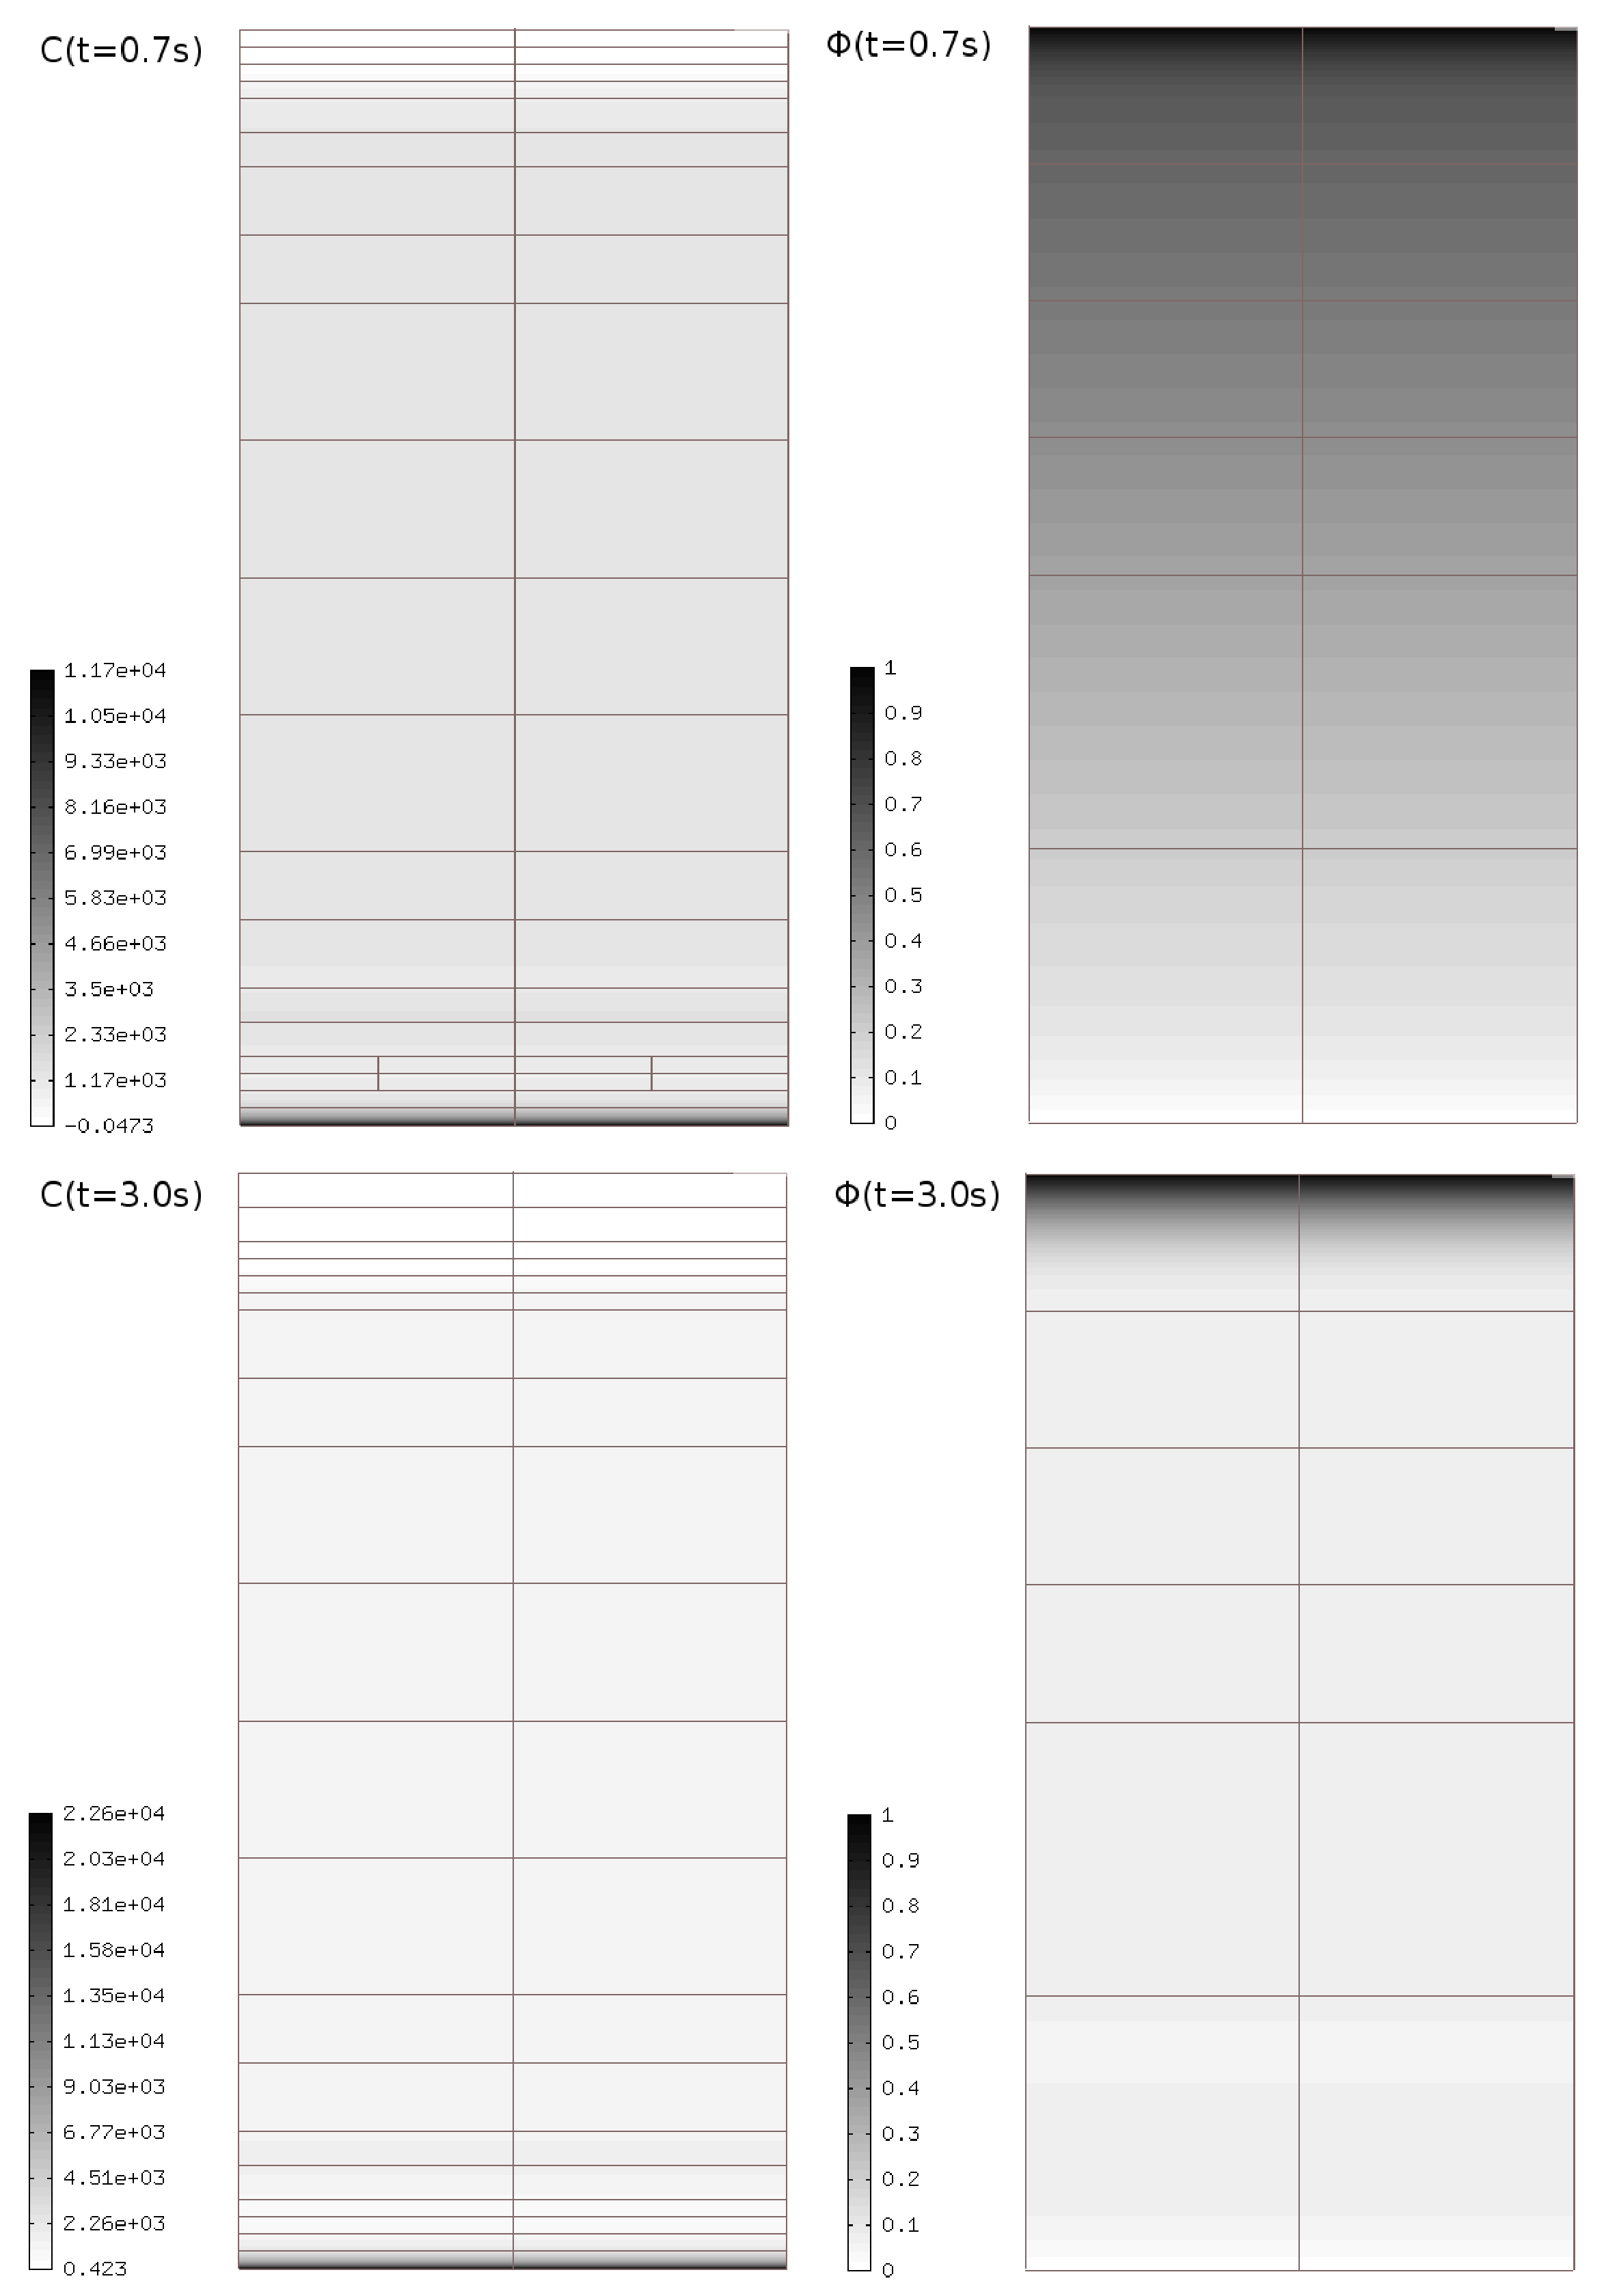
\includegraphics[width=.75\columnwidth]{cphi}
  \caption{\label{fig:cphi} Concentration $C$
  and voltage $\phi$ at two different time steps
  (HP\_ANISO adaptivity was used).}
  \end{centering}
\end{figure}
Example of the solution at $t=0.7\ s$ and $t=3.0\ s$ 
with adaptivity type HP\_ANISO is shown
in Fig.~\ref{fig:cphi}. The time $t=0.7\ s$ was chosen because
by that time, some ionic migration has already taken place, i.e.
concentration gradient near the $\partial\Omega_1$ and
$\partial\Omega_3$ has formed. The automatic mesh refinements
at different time steps are clearly visible --- especially
near the top boundary, where the concentration gradient is
moving in time (as seen in Fig.~\ref{fig:comsol-conc-volt}).

The following subsections provide a detailed comparison of
different adaptivity types and estimate the most suitable
one for the given problem.

\subsection{Optimal adaptivity types}

\begin{figure}
  \begin{centering}
  \includegraphics[width=\columnwidth]{singlemulti_dof}
  \caption{\label{fig:singlemultidof} NDOFs in case 
  of single-mesh and multi-mesh solutions with HP\_ISO
  and HP\_ANISO adaptivities. (Notice log Y scale)}
  \end{centering}
\end{figure}
\begin{figure}
  \begin{centering}
  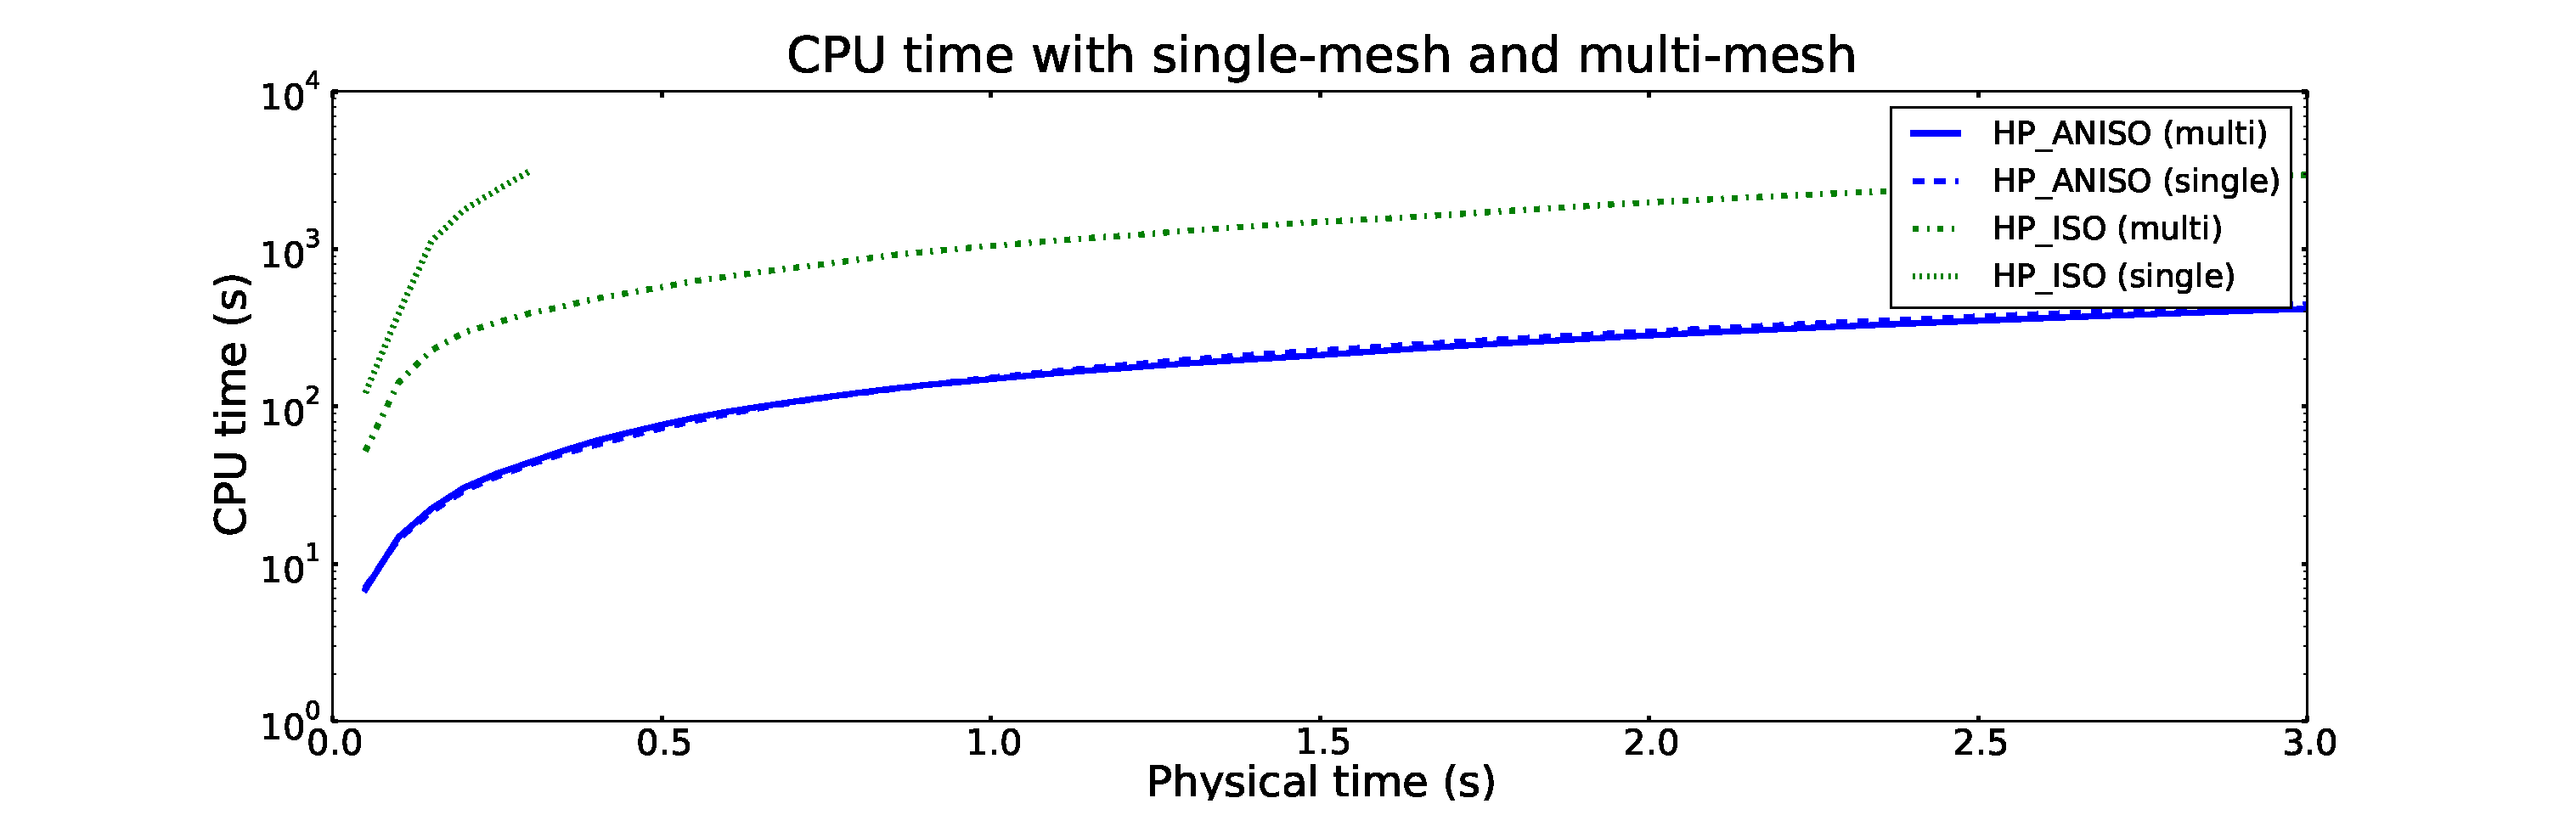
\includegraphics[width=\columnwidth]{singlemulti_cpu}
  \caption{\label{fig:singlemulticpu} CPU times in case
  of single-mesh and multi-mesh solutions with HP\_ISO
  and HP\_ANISO adaptivities. (Notice log Y scale)}
  \end{centering}
\end{figure}
\begin{figure}
  \begin{centering}
  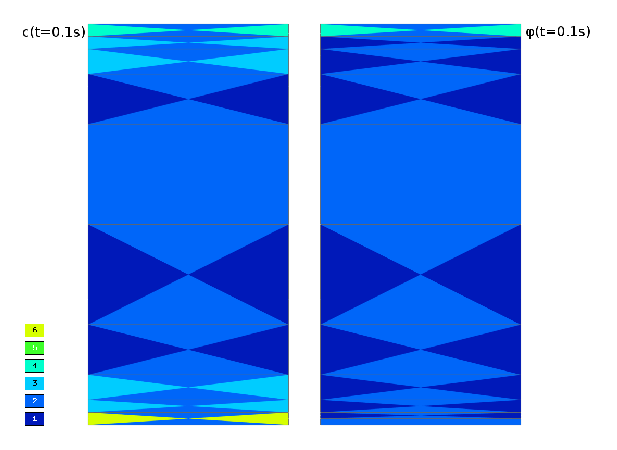
\includegraphics[width=.75\columnwidth]{poly}
  \caption{\label{fig:poly} Polynomial degree space
  for $C$ and $\phi$ at $t=0.7\ s$ The color indicates
  the maximum polynomial degree of the corresponding element.}
  \end{centering}
\end{figure}

Running the simulation with different adaptivity
types and meshes showed that the multi-mesh configuration generally results in
smaller problem size, faster calculation, and better or similar error convergence
compared to the single-mesh configuration.
This is well illustrated in Fig.~\ref{fig:singlemultidof} 
and Fig.~\ref{fig:singlemulticpu}.
This can be well understood from Fig.~\ref{fig:comsol-conc-volt} --- in the boundary
regions $\partial \Omega_1$ and $\partial\Omega_3$ the concentration gradient
is greater than voltage gradient, namely $\nabla C >> \nabla \phi$. Therefore
refining the mesh for both variables is not reasonable. For instance,
the solution space with corresponding mesh in case of
HP\_ANISO at $t=0.7\ s$ is shown in Fig.~\ref{fig:cphi}. The corresponding polynomial
degree space is shown in Fig.~\ref{fig:poly}. Notice that the adaptive algorithm
has increased the maximum polynomial degree for $C$ space to 7, however,
at the same time, maximum polynomial degree for $\phi$ is one. Furthermore,
the mesh is more refined for $C$.
For most cases using the multi-mesh results in similar or better CPU time, i.e.
multi-mesh takes less computational resources. Only excpetion was HP\_ANISO\_H 
adaptivity type for which the single mesh configuration resulted slightly faster
calculation time. 
Based on the results only multi-mesh configurations will be considered
in the following comparisons.

\begin{figure}
  \begin{centering}
  \includegraphics[width=\columnwidth]{isoaniso_dof}
  \caption{\label{fig:isoanisodof} NDOFs in case 
  of multi-mesh solutions with H\_ISO, H\_ANISO,
  HP\_ISO, HP\_ANISO, and single-mesh solution with HP\_ANISO\_H
  adaptivities. (Notice log Y scale)}
  \end{centering}
\end{figure}
\begin{figure}
  \begin{centering}
  \includegraphics[width=\columnwidth]{isoaniso_cpu}
  \caption{\label{fig:isoanisocpu} CPU times in case 
  of multi-mesh solutions with H\_ISO, H\_ANISO,
  HP\_ISO, HP\_ANISO, and single-mesh solution with HP\_ANISO\_H
  adaptivities. (notice log Y scale)}
  \end{centering}
\end{figure}
\begin{figure}
  \begin{centering}
  \includegraphics[width=\columnwidth]{isoanisop_dof}
  \caption{\label{fig:isoanisopdof} NDOFs in case 
  of multi-mesh solutions with P\_ISO, P\_ANISO, and
  HP\_ANISO\_P adaptivities.}
  \end{centering}
\end{figure}
\begin{figure}
  \begin{centering}
  \includegraphics[width=\columnwidth]{isoanisop_cpu}
  \caption{\label{fig:isoanisopcpu} CPU times in case 
  of multi-mesh solutions with P\_ISO, P\_ANISO, and
  HP\_ANISO\_P adaptivities.}
  \end{centering}
\end{figure}
To narrow down the list of adaptivity modes for the given problem, first the
isotropic and anisotropic adaptivities were compared. Here \emph{p}-adaptivity
modes are compared separately as they use more refined mesh.
Fig.~\ref{fig:isoanisodof} and Fig.~\ref{fig:isoanisocpu} show the comparison
of H\_ISO, H\_ANISO, HP\_ISO, HP\_ANISO, and HP\_ANISO\_H modes in terms of CPU time
and problem size.
Fig.~\ref{fig:isoanisopdof} and Fig.~\ref{fig:isoanisopcpu} show the similar
comparsion for the P\_ISO, P\_ANISO, and HP\_ANISO\_P modes.
Here we see that the anisotropic adaptivities result in a reasonable problem
size and the problems solve within a reasonable calculation time. It is interesting
to note that HP\_ANISO results in the smallest problem size. Also, in
\emph{p}-adaptivity group, HP\_ANISO\_P results in the smallest problem size
at each time step, whereas P\_ISO and P\_ANISO have a very largy problem size
during the first time steps of the solution.
Here the term ``reasonable problem size''
means here that the number of degrees of freedom in time converges
to so that $N_{dof}<500$, and the term ``reasonable calculation time''
means that the calculation (step $\tau=0.01\ s$, physical
time $t_{end}=3.0\ s$) time $t$ on a givem system was $t<500\ s$.
Although these parameters are empirical, they serve as an upper limit, given
that the most adaptivity modes gave significantly smaller results,
e.g. $t<<500\ s$ and $N_{dof} << 500$.

\subsection{Quantitative analysis of different adaptivity types}

Based on the results of the previous subsection, H\_ANISO, HP\_ANISO,
and HP\_ANISO\_H from the \emph{hp/h} adaptivity group and HP\_ANISO\_P
from \emph{p} adaptivity group will be compared
in terms of problem size and cumulative CPU time. 
In all of the cases, the relative 
error at each time step remained below
the threshold which were set to $e_{th}=0.5\%$ between the coarse mesh
and fine mesh solutions, therefore the error vs. time plot will not be considered.

\begin{figure}
  \begin{centering}
  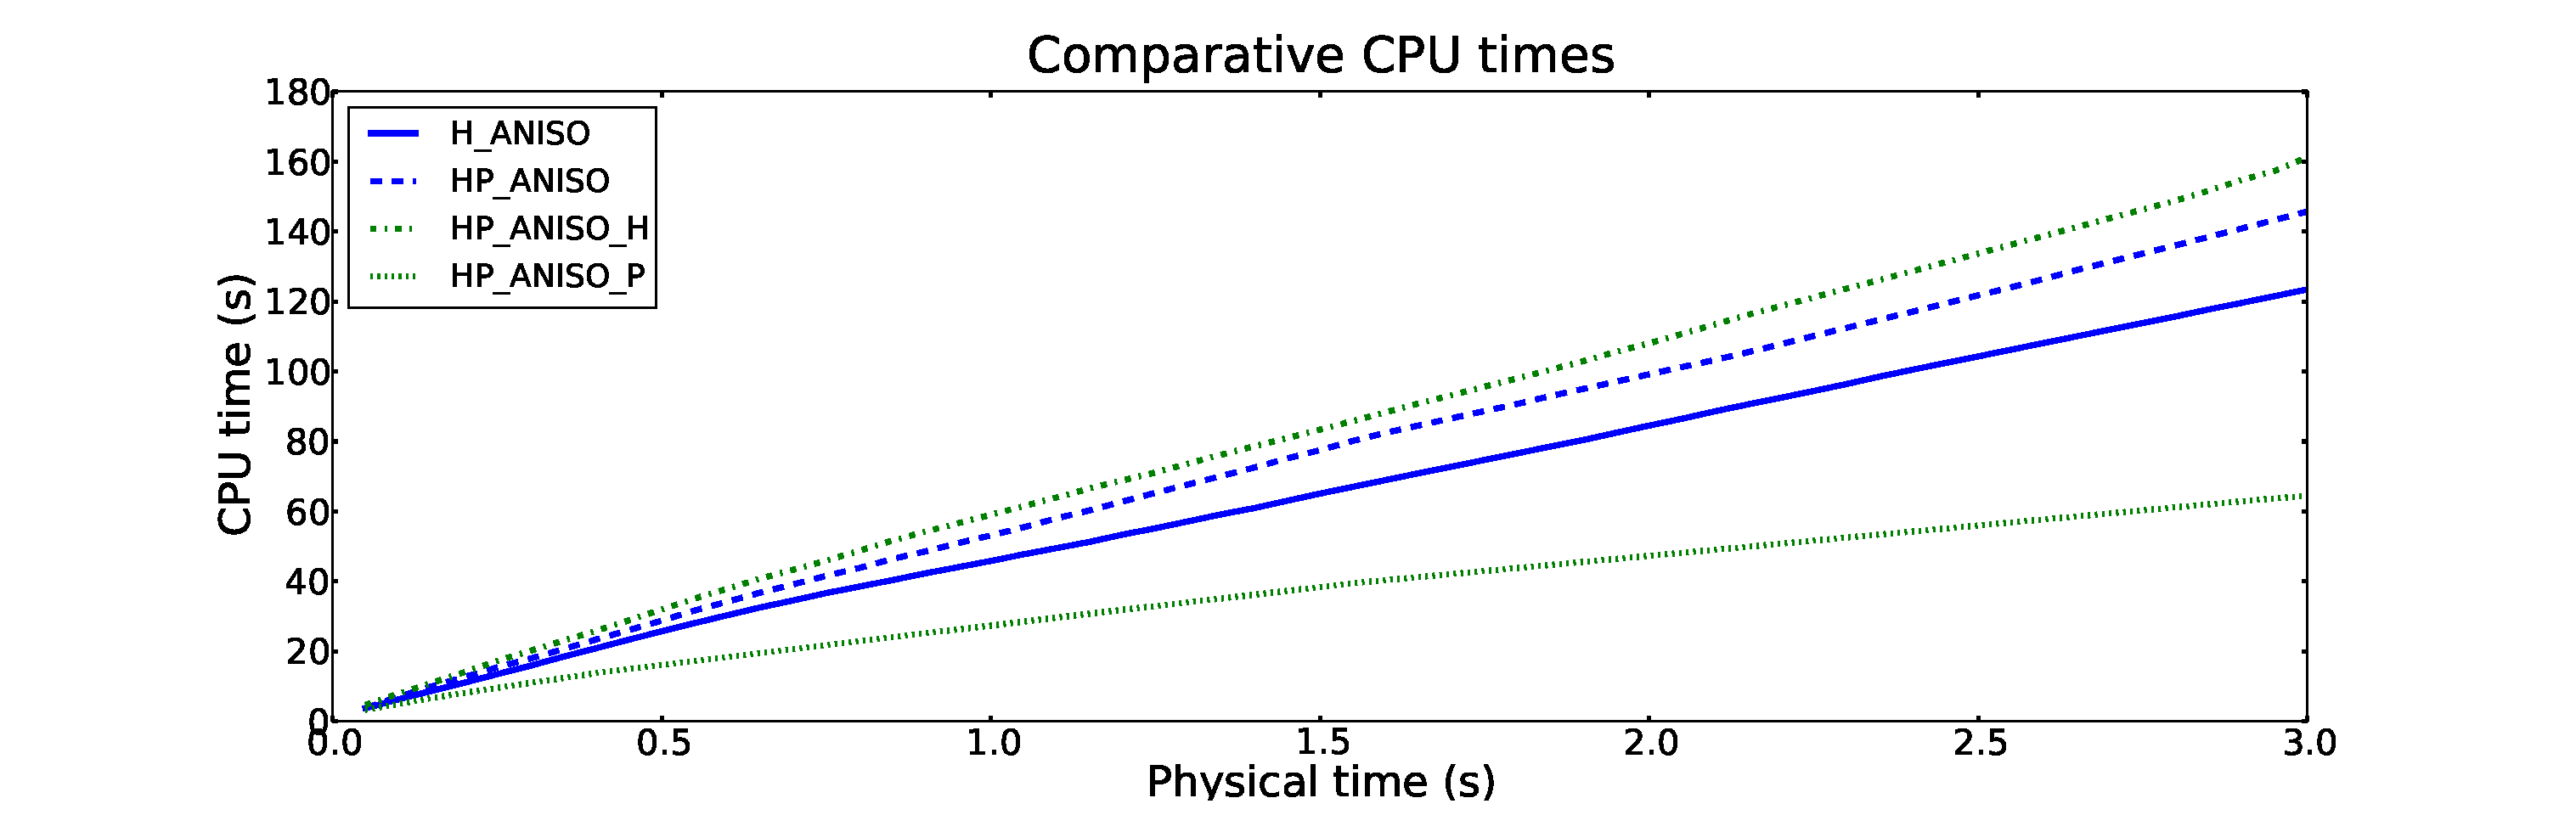
\includegraphics[width=\columnwidth]{cpu}
  \caption{\label{fig:cpu} Comparative CPU time for different adaptivity modes.}
  \end{centering}
\end{figure}

\begin{figure}
  \begin{centering}
  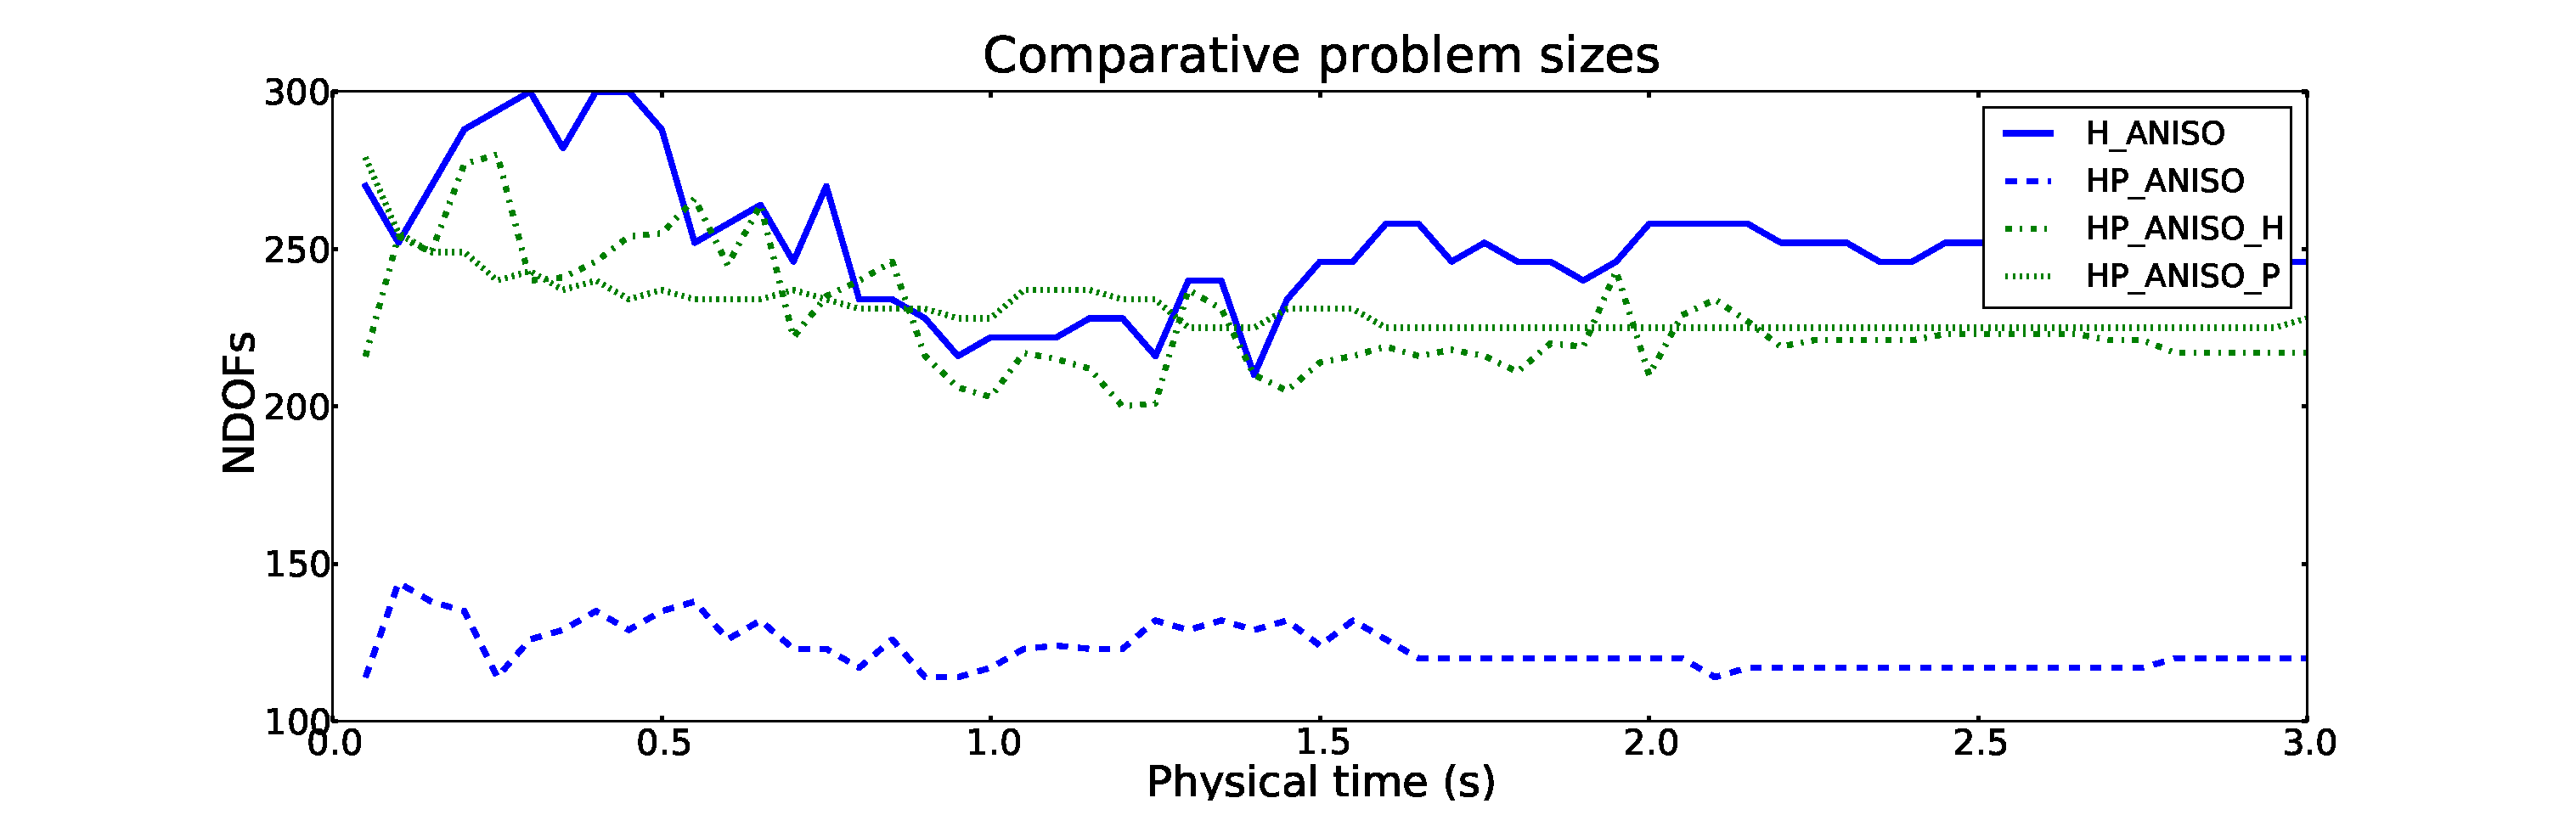
\includegraphics[width=\columnwidth]{dof}
  \caption{\label{fig:dof} Comparative NDOFs at each time step for 
  different adaptivity modes.}
  \end{centering}
\end{figure}

Fig.~\ref{fig:cpu} shows the cumulative CPU time for different adaptivity
modes at each time step. All the calculations were done on the same computer.
Here we see that HP\_ANISO\_H and HP\_ANISO require the most
resources which can be understood from the fact that these 
adaptivity modes have the largest number of 
candidates (see XXX) from which the refinement methode is chosen.
Fig.~\ref{fig:dof} shows the NDOFs at each time step for different adaptivity modes.
There we see that the HP\_ANISO results in the 
smallest problem size --- $N_{dof} \approx 125$. 
All the other adaptivity modes result in the 
problem size of approximately ($N_{dof} \approx 250$), 

\begin{figure}
  \begin{centering}
  \includegraphics[width=\columnwidth]{refined_cpu}
  \caption{\label{fig:refined-cpu} Cumulative CPU time for HP\_ANISO and HP\_ANISO\_P
  with different initial meshes.}
  \end{centering}
\end{figure}

\begin{figure}
  \begin{centering}
  \includegraphics[width=\columnwidth]{refined_dof}
  \caption{\label{fig:refined-dof} NDOFs at each time step for
  HP\_ANISO and HP\_ANISO\_P with different meshes.}
  \end{centering}
\end{figure}

So far we have seen that HP\_ANISO results in the smallest problem size, but requires
quite a lot CPU time. At the same time, HP\_ANISO\_P is the fastest, whereas
it does not result in that small problem. When it comes to a large domain 
or 3D modeling the problem
size becomes the most important factor. Therefore, we consider HP\_ANISO the most
suitable adaptivity type to the given problem. Thus some ways to optimize the time
factor will be considered.

The performance of HP\_ANISO\_P with refined mesh and half-refined
mesh, and performance of HP\_ANISO with unrefined, half-refined, and refined
meshes was calculated (see Fig.~\ref{fig:mesh}).
The results are shown in Fig.~\ref{fig:refined-cpu} and Fig.~\ref{fig:refined-dof}.

TODO(more explanation) It can be seen that some initial refinemts help to reduce the CPU time,
however, it increases the problem size.
